\section{Console Application}
Given the library \texttt{st4-scfs-sensors-1.0.0.jar} that consist of the following classes;
\texttt{CO2Sensor} - An object oriented representation of a $CO_{2}$ Sensor.
\texttt{TemperatureSensor} - An object oriented representation of a temperature
sensor.
\texttt{Test} - A class, which shows the initialisation and usage of the sensors.
Furthermore an interface \texttt{ISensor} which describes the contract that all
concrete sensors in the system should adhere to.
Any code change in the provided files are not permitted.

Given these conditions, develop a console application that can print the values
of these two sensor types.
\begin{figure}
\caption{Tree folder structure of the source code} \centering
\footnotesize
\begin{verbatim}
src/main/java/dev/nymann/
├── domain
│   ├── commands
│   │   ├── AddSensorCommand.java
│   │   ├── CommandFactory.java
│   │   ├── Command.java
│   │   ├── ICommandFactory.java
│   │   ├── ICommand.java
│   │   ├── ListSensorsCommand.java
│   │   ├── ReadSensorCommand.java
│   │   └── RemoveSensorCommand.java
│   ├── exceptions
│   │   ├── CommandExecutionException.java
│   │   └── SensorNotFoundException.java
│   └── sensors
│       ├── ISensorFactory.java
│       ├── ISensorService.java
│       ├── SensorFactory.java
│       └── SensorService.java
├── Main.java
├── presentation
│   └── Client.java
└── sensor
    ├── CO2SensorAdapter.java
    ├── ISensor.java
    ├── Sensor.java
    └── TemperatureSensorAdapter.java
\end{verbatim}
\normalsize
\end{figure}

\begin{figure}
\caption{Multilayer architecture overview}
\centering
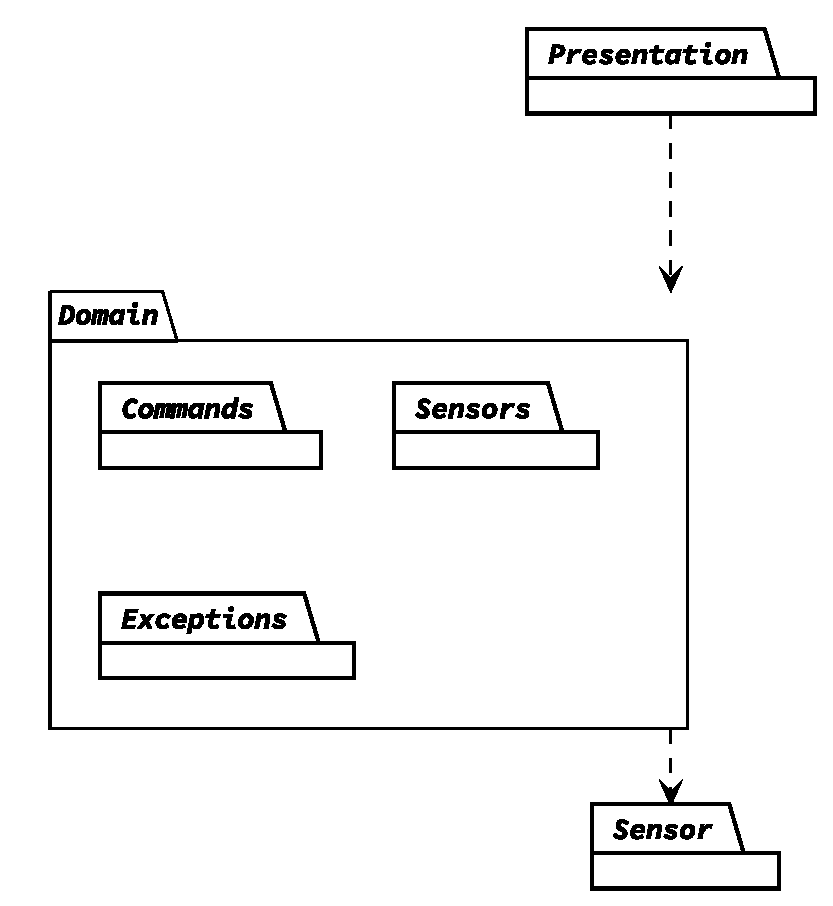
\includegraphics[scale=0.8]{part_one/components}
\end{figure}

\begin{figure}
\caption{Sensor layer class diagram}
\centering
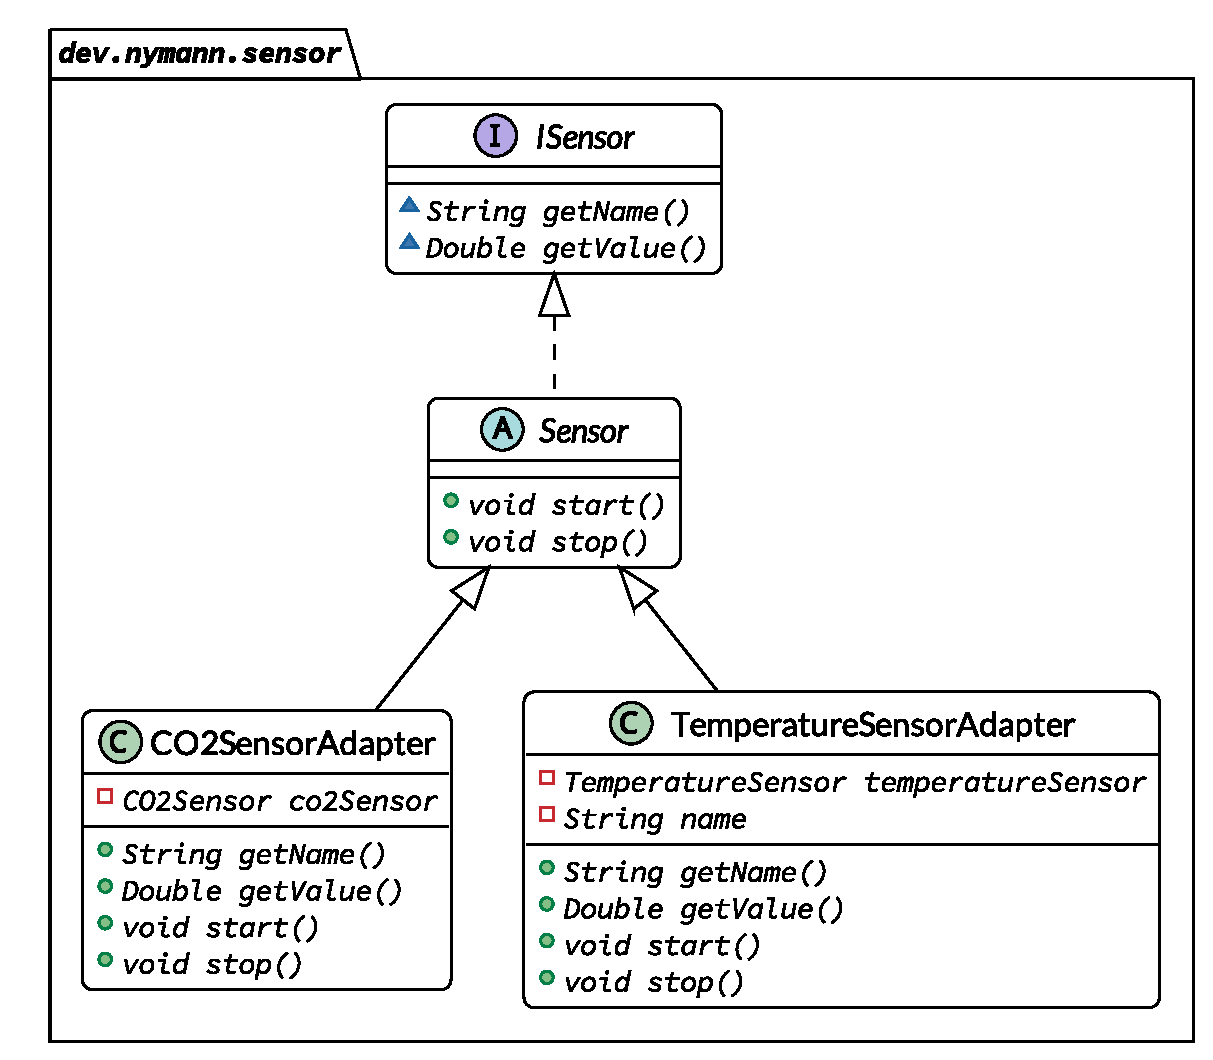
\includegraphics[width=1\textwidth]{part_one/sensor}
\end{figure}

\begin{figure}
\caption{Commands package in the domain layer}
\centering
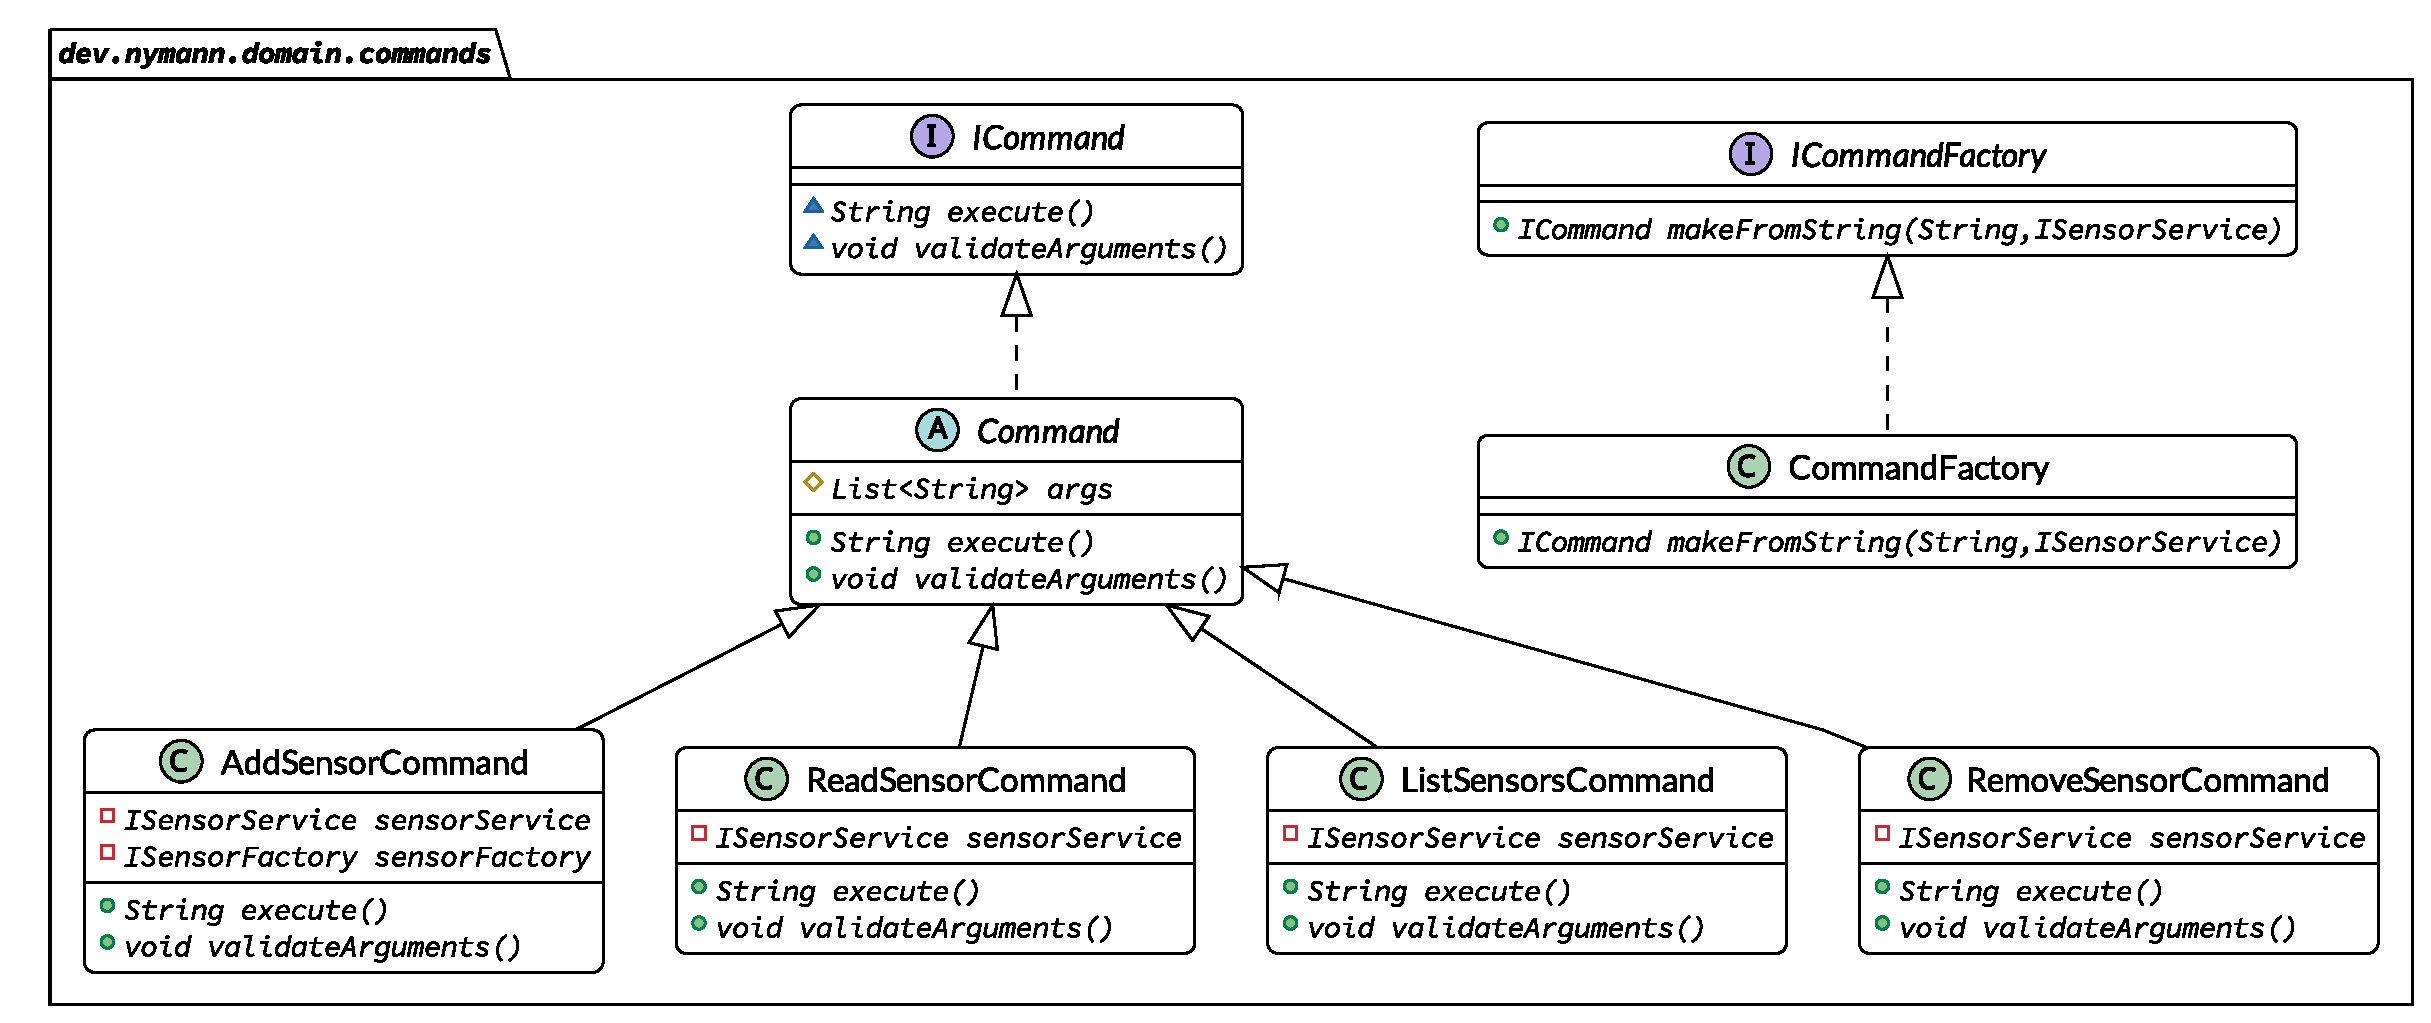
\includegraphics[width=1\textwidth]{part_one/domain-commands}
\end{figure}

\begin{figure}
\caption{Sensors package in the domain layer}
\centering
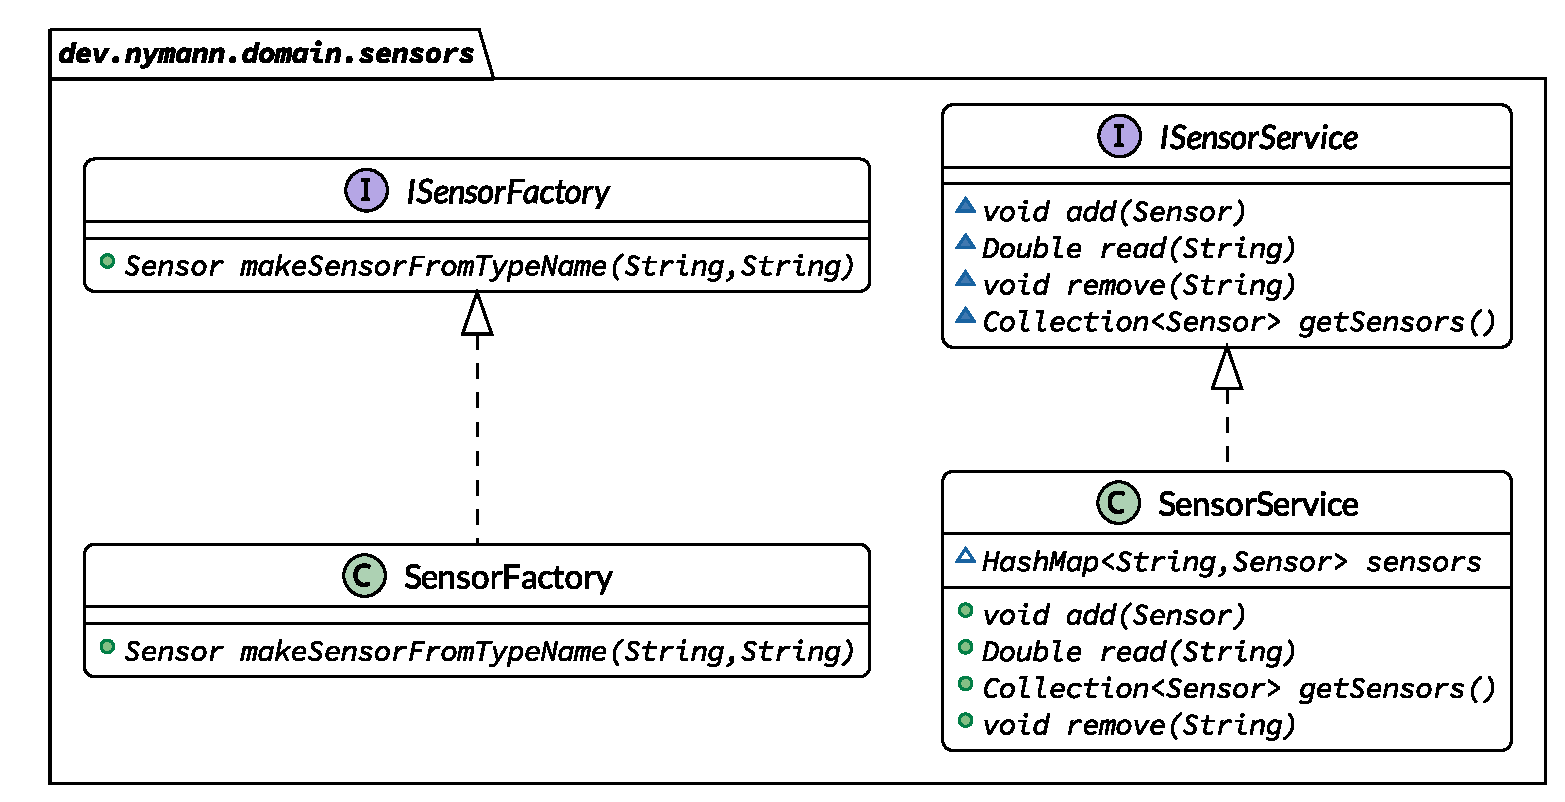
\includegraphics[width=1\textwidth]{part_one/domain-sensors}
\end{figure}

\begin{figure}
\caption{Exceptions package in the domain layer }
\centering
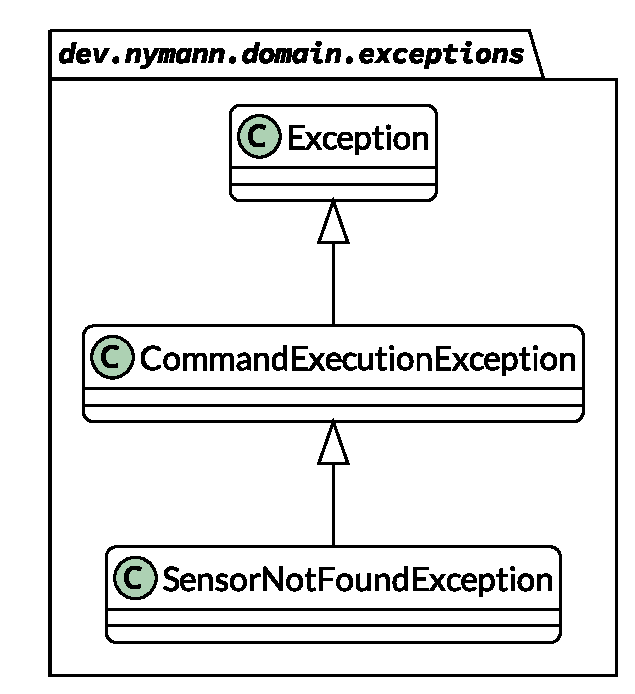
\includegraphics[width=0.4\textwidth]{part_one/domain-exceptions}
\end{figure}

\begin{figure}
\caption{Presentation layer class diagram}
\centering
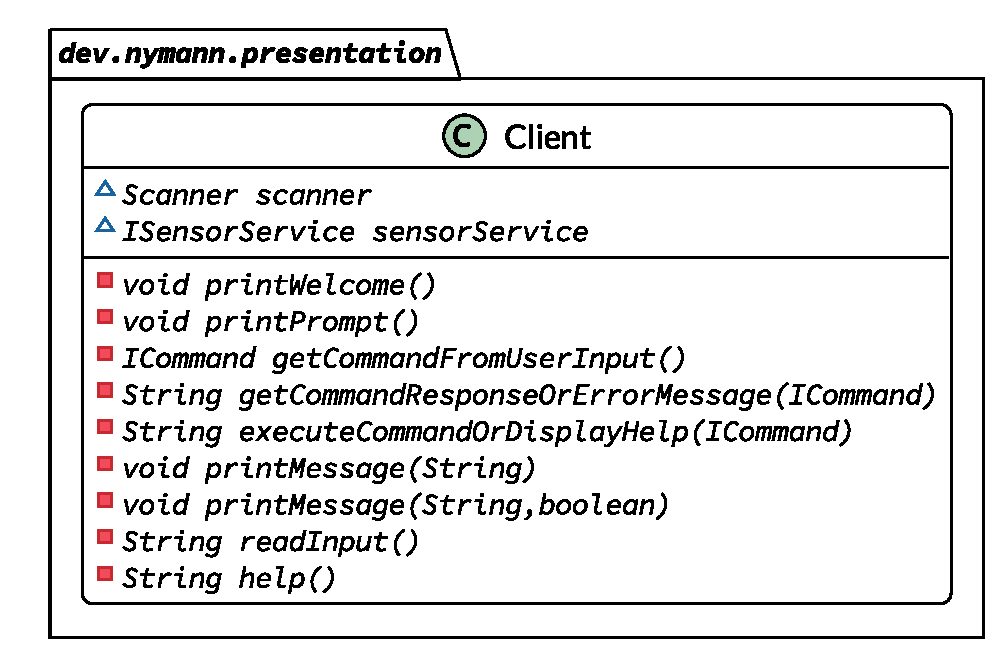
\includegraphics[width=1\textwidth]{part_one/presentation}
\end{figure}
